%\documentclass[english,utf8,10pt,t]{beamer}
\documentclass[aspectratio=169]{beamer}
\usepackage{graphicx}

\mode<presentation>{
\usetheme{TUMCD2015SEC}
}

%\usepackage{listings}
%\usepackage{xcolor}
%\usepackage{capt-of}
%\usepackage{units}
%\usepackage{graphicx}
%\usepackage{url}
%\usepackage{amsmath}
%\usepackage{amssymb}
%\usepackage{booktabs}
%\usepackage{threeparttable}

%\usepackage{tikz}
%\usetikzlibrary{backgrounds,patterns,decorations,positioning}
%\usetikzlibrary{decorations.pathmorphing}
%\usepgfmodule{decorations}

\title[Short Title]{Analysis of Machine Learning for State Register Identification}
\subtitle{Bachelor's Thesis}
%\subtitle{Subtitle}
\author[Lee Seng Hwee]{\underline{Lee Seng Hwee}}
\institute[TUM]{\inst{1}Technische Universit{\"a}t M{\"u}nchen\\Faculty of Electrical and Computer Engineering\\Institute for Security in Information Technology\and University}
\date{\today}
\begin{document}


\begin{frame}
	\titlepage
\end{frame}

\section*{Outline}
\begin{frame}{Outline}
\tableofcontents
\end{frame}

\section{Introduction}
\begin{frame}{Introduction}
\textbf{Limitation of Current Approaches}
\medskip\newline
Traditional approach:
\medskip
\begin{itemize}
	\item Requires golden model
\end{itemize}

\bigskip
RELIC and fastRELIC:
\medskip
\begin{itemize}
	\item Based solely on Pair Similarity Score(PSS)
\end{itemize}
\end{frame}

\section{Problem Statement}
\begin{frame}{Problem Statement}
\begin{center}
	\emph{Reliance on a golden model in the traditional method results in severe identification limitations, while RELIC/fastRELIC which relied solely on PSS, results in a lower accuracy.}
\end{center}
\end{frame}

\section{Proposed Solution}
\begin{frame}{Proposed Solution}
To train and deploy a machine learning model for State Register identification.
\bigskip\newline
Advantages of Machine Learning:
\begin{itemize}
	\item Faster Processing
	\item Ease of use
	\item Consistency in evaluation
	\item Rely on multiple features 
\end{itemize}
\end{frame}

\section{Implementations}
\begin{frame}[c]{ }
	\begin{center}
		\Huge Implementations
	\end{center}
\end{frame}


\begin{frame}{The Data}
Prior to creating a Neural Network for State Register Identification, 4 methods of implementating the feature file was discussed for training the Neural Network
\bigskip\begin{itemize}
	\item Original features set
	\item Original features set with Euclidean Distance Similarity Score
	\item Original features set with fastRELIC Similarity Score
	\item Original features set with Euclidean and fastRELIC Similarity Score
\end{itemize}
\end{frame}

\begin{frame}{The Original Features}
\begin{table}
		\begin{tabular}{|c|c|}
		\hline
		Average Neighbour Degree & Betweenness Centrality\\
		\hline
		Closeness Centrality & Clustering\\
		\hline
		Degree & Degree Centrality\\
		\hline
		Indegree & Has Feedback Path\\
		\hline
		Katz & Load Centrality\\
		\hline
		Outdegree & Pagerank\\
		\hline
	\end{tabular}
	\caption{Original Features}
	\label{tab:Original Features}
\end{table}

\end{frame}

\begin{frame}{Euclidean Distance Similarity Score}
\begin{itemize}
	\item By extracting Register Shapes from design files
\end{itemize}
\begin{figure}
	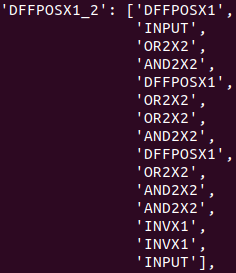
\includegraphics[scale=0.5]{./Results/vector/shape_vector_1.png}
	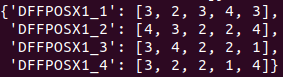
\includegraphics[scale=0.5]{./Results/vector/vector.png}
\end{figure}
\end{frame}

\begin{frame}{Euclidean Distance Similarity Score}
\begin{itemize}
	\item Comparing vectors, producing a similarity score using Euclidean Distance
\end{itemize}
\begin{equation*}
\label{eqn:euclidean distance nth dimension}
E(u, v)=\sqrt{\sum_{i=1}^{n} {(u_{i} - v_{i})^2}}
\end{equation*}
where $u$ and $v$ are $n^{th}$-dimensional vectors

\begin{itemize}
	\item Count++, if $E(u, v)<Threshold$
	\item Normalize
\end{itemize}

\end{frame}

\begin{frame}{fastRELIC Similarity Score}
\begin{itemize}
	\item Using PSS algorithm, similarity score between 0 to 1
	\item Count++, if $PSS>Threshold$
	\item Normalize
\end{itemize}
\end{frame}

\begin{frame}{Features Selection}
\textbf{Constant Filtering}
\begin{itemize}
	\item Removing features with constant values
\end{itemize}
\textit{\textbf{Quasi-constant filtering}
\begin{itemize}
	\item Removing features with a value difference less than a selected threshold
\end{itemize}}
\textbf{Feature Permutation}
\begin{itemize}
	\item Permutes the values in a feature 
	\item Trains data set with the permuted feature on pre-optimised neural network
	\item Compare permuted accuracy with unpermuted accuracy
\end{itemize}
\textbf{Sequential Feature Selection}
\begin{itemize}
	\item Train on pre-optimised neural network
	\item Select feature combinations based on accuracy by adding features one at a time
\end{itemize}
\end{frame}

\section{Methodology and Results}
\begin{frame}[c]{ }
\begin{center}
	\Huge Methodology and Results
\end{center}
\end{frame}

\begin{frame}{Testing Implementaion (Pre-Optimize Neural Network)}
\begin{itemize}
	\item Rotation of 13 files, 12 for training, 1 for testing
		\begin{itemize}
			\item Train with files B -- N, test with file A
			\item Train with files A, C -- N, test with file B
		\end{itemize}
	\item Per file was used to train the model 100 times, experiment repeated 5 times
	\item Average result per implementation across all 13 tests
       \begin{equation*}
           \label{eqn:model accuracy equation}
           \text{A}= \frac{\text{Number of Correctly Predicted Registers}}{\text{Total Number of Registers}}
       \end{equation*}

       \begin{equation*}
       \label{eqn:state register prediction accuracy equation}
       \text{SRA}= \frac{\text{Number of Correctly Predicted State Registers}}{\text{Total Number of State Registers}}
       \end{equation*}
\end{itemize}
\end{frame}

\begin{frame}{Results for different implementation}
\centering
\begin{table}
	\begin{tabular}{|c|c|c|}
		\hline
		Implementation & Mean Model Acc & Mean State Register Acc \\
		\hline
		\hline
		Original & 0.75 & 0.59\\
		\hline
		With fastRELIC & 0.86 & 0.77\\
		\hline
		With Euclidean & 0.83 & 0.71\\
		\hline
		With Euclidean and fastRELIC & 0.87 & 0.78\\
		\hline
	\end{tabular}
	\caption{Accuracy}
	\label{tab:Accuracy No Feature Selection}
\end{table}
\end{frame}


\begin{frame}{Feature Permutation Methodology}
\begin{itemize}
	\item Rotation of 13 files, 12 for training, 1 for testing
	\item Each feature in a file permuted individually and train the model for 100 times
	\item Average the 100 accuracies per features
	\item Train model with non-permuted data set for 100 times and calculate average
	\item Repeat experiment for 5 times
	\item Calculate Ratio(Method 1) and Feature Occurrence(Method 2)
\end{itemize}
\end{frame}

\begin{frame}{Ratio --- Method 1}
\begin{equation*}
	\label{eqn:ratio model accuracy}
   R_n(A_{original}, A_{permuted})= \frac{A_{original}}{A_{permuted}}
\end{equation*}
\begin{equation*}
   \label{ration state register accuracy}
   SRR_n(SRA_{original}, SRA_{permuted})= \frac{SRA_{original}}{SRA_{permuted}}
\end{equation*}
\begin{table}[ht]
	\centering
   \begin{tabular}{|c|c|c|}
   	\hline
   	$R_n<1$ & $SRR_n<1$ & Feature Hindrance\\
   	\hline
  		$R_n=1$ & $SRR_n=1$ & Feature Hindrance\\
   	\hline
   	$R_n>1$ & $SRR_n>1$ & Feature Important\\
   	\hline
   \end{tabular}
   \caption{Ratio Interpretation}
   \label{tab: Ratio Interpretation}
\end{table}
\end{frame}

\begin{frame}{Feature Permutation Method 1 \\Model Accuracy Ratio}
\centering
\resizebox{!}{0.7\paperheight}{
	% GNUPLOT: LaTeX picture with Postscript
\begingroup
  \makeatletter
  \providecommand\color[2][]{%
    \GenericError{(gnuplot) \space\space\space\@spaces}{%
      Package color not loaded in conjunction with
      terminal option `colourtext'%
    }{See the gnuplot documentation for explanation.%
    }{Either use 'blacktext' in gnuplot or load the package
      color.sty in LaTeX.}%
    \renewcommand\color[2][]{}%
  }%
  \providecommand\includegraphics[2][]{%
    \GenericError{(gnuplot) \space\space\space\@spaces}{%
      Package graphicx or graphics not loaded%
    }{See the gnuplot documentation for explanation.%
    }{The gnuplot epslatex terminal needs graphicx.sty or graphics.sty.}%
    \renewcommand\includegraphics[2][]{}%
  }%
  \providecommand\rotatebox[2]{#2}%
  \@ifundefined{ifGPcolor}{%
    \newif\ifGPcolor
    \GPcolortrue
  }{}%
  \@ifundefined{ifGPblacktext}{%
    \newif\ifGPblacktext
    \GPblacktexttrue
  }{}%
  % define a \g@addto@macro without @ in the name:
  \let\gplgaddtomacro\g@addto@macro
  % define empty templates for all commands taking text:
  \gdef\gplbacktext{}%
  \gdef\gplfronttext{}%
  \makeatother
  \ifGPblacktext
    % no textcolor at all
    \def\colorrgb#1{}%
    \def\colorgray#1{}%
  \else
    % gray or color?
    \ifGPcolor
      \def\colorrgb#1{\color[rgb]{#1}}%
      \def\colorgray#1{\color[gray]{#1}}%
      \expandafter\def\csname LTw\endcsname{\color{white}}%
      \expandafter\def\csname LTb\endcsname{\color{black}}%
      \expandafter\def\csname LTa\endcsname{\color{black}}%
      \expandafter\def\csname LT0\endcsname{\color[rgb]{1,0,0}}%
      \expandafter\def\csname LT1\endcsname{\color[rgb]{0,1,0}}%
      \expandafter\def\csname LT2\endcsname{\color[rgb]{0,0,1}}%
      \expandafter\def\csname LT3\endcsname{\color[rgb]{1,0,1}}%
      \expandafter\def\csname LT4\endcsname{\color[rgb]{0,1,1}}%
      \expandafter\def\csname LT5\endcsname{\color[rgb]{1,1,0}}%
      \expandafter\def\csname LT6\endcsname{\color[rgb]{0,0,0}}%
      \expandafter\def\csname LT7\endcsname{\color[rgb]{1,0.3,0}}%
      \expandafter\def\csname LT8\endcsname{\color[rgb]{0.5,0.5,0.5}}%
    \else
      % gray
      \def\colorrgb#1{\color{black}}%
      \def\colorgray#1{\color[gray]{#1}}%
      \expandafter\def\csname LTw\endcsname{\color{white}}%
      \expandafter\def\csname LTb\endcsname{\color{black}}%
      \expandafter\def\csname LTa\endcsname{\color{black}}%
      \expandafter\def\csname LT0\endcsname{\color{black}}%
      \expandafter\def\csname LT1\endcsname{\color{black}}%
      \expandafter\def\csname LT2\endcsname{\color{black}}%
      \expandafter\def\csname LT3\endcsname{\color{black}}%
      \expandafter\def\csname LT4\endcsname{\color{black}}%
      \expandafter\def\csname LT5\endcsname{\color{black}}%
      \expandafter\def\csname LT6\endcsname{\color{black}}%
      \expandafter\def\csname LT7\endcsname{\color{black}}%
      \expandafter\def\csname LT8\endcsname{\color{black}}%
    \fi
  \fi
    \setlength{\unitlength}{0.0500bp}%
    \ifx\gptboxheight\undefined%
      \newlength{\gptboxheight}%
      \newlength{\gptboxwidth}%
      \newsavebox{\gptboxtext}%
    \fi%
    \setlength{\fboxrule}{0.5pt}%
    \setlength{\fboxsep}{1pt}%
\begin{picture}(9636.00,6802.00)%
    \gplgaddtomacro\gplbacktext{%
      \csname LTb\endcsname%%
      \put(726,1803){\makebox(0,0)[r]{\strut{}$0.9$}}%
      \csname LTb\endcsname%%
      \put(726,2400){\makebox(0,0)[r]{\strut{}$0.95$}}%
      \csname LTb\endcsname%%
      \put(726,2998){\makebox(0,0)[r]{\strut{}$1$}}%
      \csname LTb\endcsname%%
      \put(726,3595){\makebox(0,0)[r]{\strut{}$1.05$}}%
      \csname LTb\endcsname%%
      \put(726,4192){\makebox(0,0)[r]{\strut{}$1.1$}}%
      \csname LTb\endcsname%%
      \put(726,4789){\makebox(0,0)[r]{\strut{}$1.15$}}%
      \csname LTb\endcsname%%
      \put(726,5387){\makebox(0,0)[r]{\strut{}$1.2$}}%
      \csname LTb\endcsname%%
      \put(726,5984){\makebox(0,0)[r]{\strut{}$1.25$}}%
      \csname LTb\endcsname%%
      \put(726,6581){\makebox(0,0)[r]{\strut{}$1.3$}}%
      \csname LTb\endcsname%%
      \put(1975,1671){\rotatebox{30}{\makebox(0,0)[r]{\strut{}average neighbour degree}}}%
      \csname LTb\endcsname%%
      \put(2534,1671){\rotatebox{30}{\makebox(0,0)[r]{\strut{}betweenness centrality}}}%
      \csname LTb\endcsname%%
      \put(3093,1671){\rotatebox{30}{\makebox(0,0)[r]{\strut{}closeness centrality}}}%
      \csname LTb\endcsname%%
      \put(3652,1671){\rotatebox{30}{\makebox(0,0)[r]{\strut{}clustering}}}%
      \csname LTb\endcsname%%
      \put(4210,1671){\rotatebox{30}{\makebox(0,0)[r]{\strut{}degree}}}%
      \csname LTb\endcsname%%
      \put(4769,1671){\rotatebox{30}{\makebox(0,0)[r]{\strut{}degree centrality}}}%
      \csname LTb\endcsname%%
      \put(5328,1671){\rotatebox{30}{\makebox(0,0)[r]{\strut{}has feedback path}}}%
      \csname LTb\endcsname%%
      \put(5887,1671){\rotatebox{30}{\makebox(0,0)[r]{\strut{}katz}}}%
      \csname LTb\endcsname%%
      \put(6445,1671){\rotatebox{30}{\makebox(0,0)[r]{\strut{}load centrality}}}%
      \csname LTb\endcsname%%
      \put(7004,1671){\rotatebox{30}{\makebox(0,0)[r]{\strut{}outdegree}}}%
      \csname LTb\endcsname%%
      \put(7563,1671){\rotatebox{30}{\makebox(0,0)[r]{\strut{}pagerank}}}%
      \csname LTb\endcsname%%
      \put(8122,1671){\rotatebox{30}{\makebox(0,0)[r]{\strut{}Euclidean}}}%
      \csname LTb\endcsname%%
      \put(8680,1671){\rotatebox{30}{\makebox(0,0)[r]{\strut{}fastRELIC}}}%
    }%
    \gplgaddtomacro\gplfronttext{%
      \csname LTb\endcsname%%
      \put(8252,6408){\makebox(0,0)[r]{\strut{}Orignal}}%
      \csname LTb\endcsname%%
      \put(8252,6188){\makebox(0,0)[r]{\strut{}With fastRELIC}}%
      \csname LTb\endcsname%%
      \put(8252,5968){\makebox(0,0)[r]{\strut{}With Euclidean}}%
      \csname LTb\endcsname%%
      \put(8252,5748){\makebox(0,0)[r]{\strut{}With Euclidean and fastRELIC}}%
    }%
    \gplbacktext
    \put(0,0){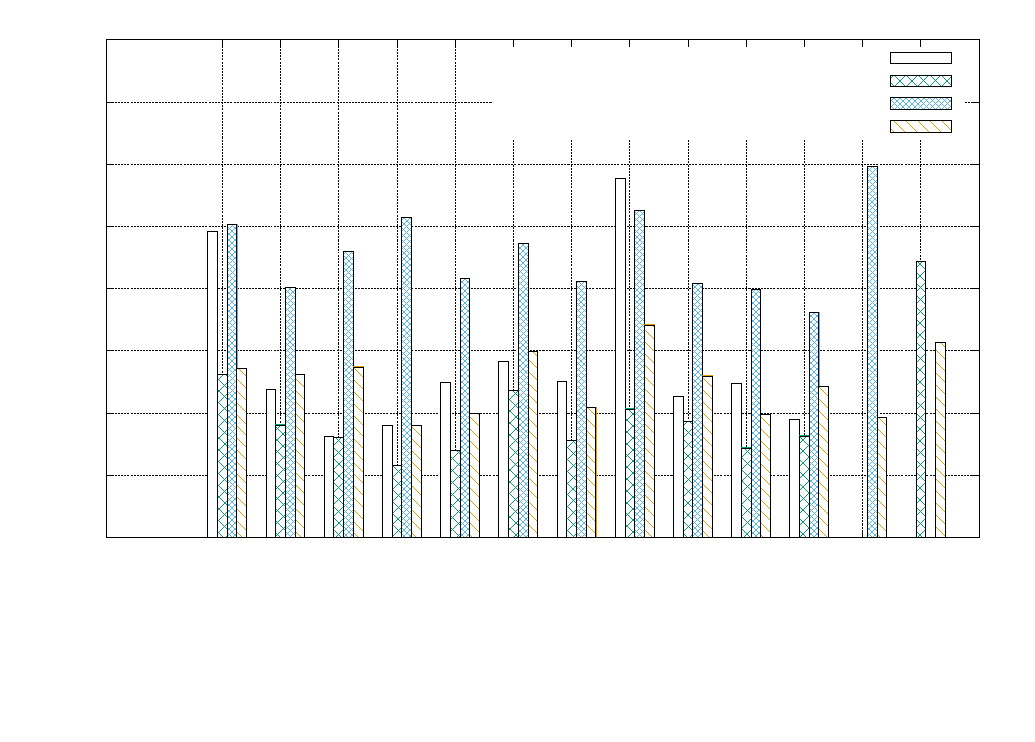
\includegraphics{myFiles/myLatex/Feature_Permutation/FeaturePermutation_ratio.eps}}%
    \gplfronttext
  \end{picture}%
\endgroup

	\label{fig:Model Accuracy Ratio ($R_n$) Per Feature}
}
\end{frame}

\begin{frame}{Feature Permutation Method 1 \\State Register Accuracy Ratio}
\centering
\resizebox{!}{0.7\paperheight}{
	% GNUPLOT: LaTeX picture with Postscript
\begingroup
  \makeatletter
  \providecommand\color[2][]{%
    \GenericError{(gnuplot) \space\space\space\@spaces}{%
      Package color not loaded in conjunction with
      terminal option `colourtext'%
    }{See the gnuplot documentation for explanation.%
    }{Either use 'blacktext' in gnuplot or load the package
      color.sty in LaTeX.}%
    \renewcommand\color[2][]{}%
  }%
  \providecommand\includegraphics[2][]{%
    \GenericError{(gnuplot) \space\space\space\@spaces}{%
      Package graphicx or graphics not loaded%
    }{See the gnuplot documentation for explanation.%
    }{The gnuplot epslatex terminal needs graphicx.sty or graphics.sty.}%
    \renewcommand\includegraphics[2][]{}%
  }%
  \providecommand\rotatebox[2]{#2}%
  \@ifundefined{ifGPcolor}{%
    \newif\ifGPcolor
    \GPcolortrue
  }{}%
  \@ifundefined{ifGPblacktext}{%
    \newif\ifGPblacktext
    \GPblacktexttrue
  }{}%
  % define a \g@addto@macro without @ in the name:
  \let\gplgaddtomacro\g@addto@macro
  % define empty templates for all commands taking text:
  \gdef\gplbacktext{}%
  \gdef\gplfronttext{}%
  \makeatother
  \ifGPblacktext
    % no textcolor at all
    \def\colorrgb#1{}%
    \def\colorgray#1{}%
  \else
    % gray or color?
    \ifGPcolor
      \def\colorrgb#1{\color[rgb]{#1}}%
      \def\colorgray#1{\color[gray]{#1}}%
      \expandafter\def\csname LTw\endcsname{\color{white}}%
      \expandafter\def\csname LTb\endcsname{\color{black}}%
      \expandafter\def\csname LTa\endcsname{\color{black}}%
      \expandafter\def\csname LT0\endcsname{\color[rgb]{1,0,0}}%
      \expandafter\def\csname LT1\endcsname{\color[rgb]{0,1,0}}%
      \expandafter\def\csname LT2\endcsname{\color[rgb]{0,0,1}}%
      \expandafter\def\csname LT3\endcsname{\color[rgb]{1,0,1}}%
      \expandafter\def\csname LT4\endcsname{\color[rgb]{0,1,1}}%
      \expandafter\def\csname LT5\endcsname{\color[rgb]{1,1,0}}%
      \expandafter\def\csname LT6\endcsname{\color[rgb]{0,0,0}}%
      \expandafter\def\csname LT7\endcsname{\color[rgb]{1,0.3,0}}%
      \expandafter\def\csname LT8\endcsname{\color[rgb]{0.5,0.5,0.5}}%
    \else
      % gray
      \def\colorrgb#1{\color{black}}%
      \def\colorgray#1{\color[gray]{#1}}%
      \expandafter\def\csname LTw\endcsname{\color{white}}%
      \expandafter\def\csname LTb\endcsname{\color{black}}%
      \expandafter\def\csname LTa\endcsname{\color{black}}%
      \expandafter\def\csname LT0\endcsname{\color{black}}%
      \expandafter\def\csname LT1\endcsname{\color{black}}%
      \expandafter\def\csname LT2\endcsname{\color{black}}%
      \expandafter\def\csname LT3\endcsname{\color{black}}%
      \expandafter\def\csname LT4\endcsname{\color{black}}%
      \expandafter\def\csname LT5\endcsname{\color{black}}%
      \expandafter\def\csname LT6\endcsname{\color{black}}%
      \expandafter\def\csname LT7\endcsname{\color{black}}%
      \expandafter\def\csname LT8\endcsname{\color{black}}%
    \fi
  \fi
    \setlength{\unitlength}{0.0500bp}%
    \ifx\gptboxheight\undefined%
      \newlength{\gptboxheight}%
      \newlength{\gptboxwidth}%
      \newsavebox{\gptboxtext}%
    \fi%
    \setlength{\fboxrule}{0.5pt}%
    \setlength{\fboxsep}{1pt}%
\begin{picture}(9636.00,6802.00)%
    \gplgaddtomacro\gplbacktext{%
      \csname LTb\endcsname%%
      \put(594,1803){\makebox(0,0)[r]{\strut{}$0.5$}}%
      \csname LTb\endcsname%%
      \put(594,2998){\makebox(0,0)[r]{\strut{}$1$}}%
      \csname LTb\endcsname%%
      \put(594,4192){\makebox(0,0)[r]{\strut{}$1.5$}}%
      \csname LTb\endcsname%%
      \put(594,5387){\makebox(0,0)[r]{\strut{}$2$}}%
      \csname LTb\endcsname%%
      \put(594,6581){\makebox(0,0)[r]{\strut{}$2.5$}}%
      \csname LTb\endcsname%%
      \put(1861,1671){\rotatebox{30}{\makebox(0,0)[r]{\strut{}average neighbour degree}}}%
      \csname LTb\endcsname%%
      \put(2429,1671){\rotatebox{30}{\makebox(0,0)[r]{\strut{}betweenness centrality}}}%
      \csname LTb\endcsname%%
      \put(2996,1671){\rotatebox{30}{\makebox(0,0)[r]{\strut{}closeness centrality}}}%
      \csname LTb\endcsname%%
      \put(3564,1671){\rotatebox{30}{\makebox(0,0)[r]{\strut{}clustering}}}%
      \csname LTb\endcsname%%
      \put(4131,1671){\rotatebox{30}{\makebox(0,0)[r]{\strut{}degree}}}%
      \csname LTb\endcsname%%
      \put(4699,1671){\rotatebox{30}{\makebox(0,0)[r]{\strut{}degree centrality}}}%
      \csname LTb\endcsname%%
      \put(5266,1671){\rotatebox{30}{\makebox(0,0)[r]{\strut{}has feedback path}}}%
      \csname LTb\endcsname%%
      \put(5834,1671){\rotatebox{30}{\makebox(0,0)[r]{\strut{}katz}}}%
      \csname LTb\endcsname%%
      \put(6401,1671){\rotatebox{30}{\makebox(0,0)[r]{\strut{}load centrality}}}%
      \csname LTb\endcsname%%
      \put(6969,1671){\rotatebox{30}{\makebox(0,0)[r]{\strut{}outdegree}}}%
      \csname LTb\endcsname%%
      \put(7536,1671){\rotatebox{30}{\makebox(0,0)[r]{\strut{}pagerank}}}%
      \csname LTb\endcsname%%
      \put(8104,1671){\rotatebox{30}{\makebox(0,0)[r]{\strut{}euclidean}}}%
      \csname LTb\endcsname%%
      \put(8671,1671){\rotatebox{30}{\makebox(0,0)[r]{\strut{}fastRELIC}}}%
    }%
    \gplgaddtomacro\gplfronttext{%
      \csname LTb\endcsname%%
      \put(8252,6408){\makebox(0,0)[r]{\strut{}Original}}%
      \csname LTb\endcsname%%
      \put(8252,6188){\makebox(0,0)[r]{\strut{}With fastRELIC}}%
      \csname LTb\endcsname%%
      \put(8252,5968){\makebox(0,0)[r]{\strut{}With Euclidean}}%
      \csname LTb\endcsname%%
      \put(8252,5748){\makebox(0,0)[r]{\strut{}With Euclidean and fastRELIC}}%
    }%
    \gplbacktext
    \put(0,0){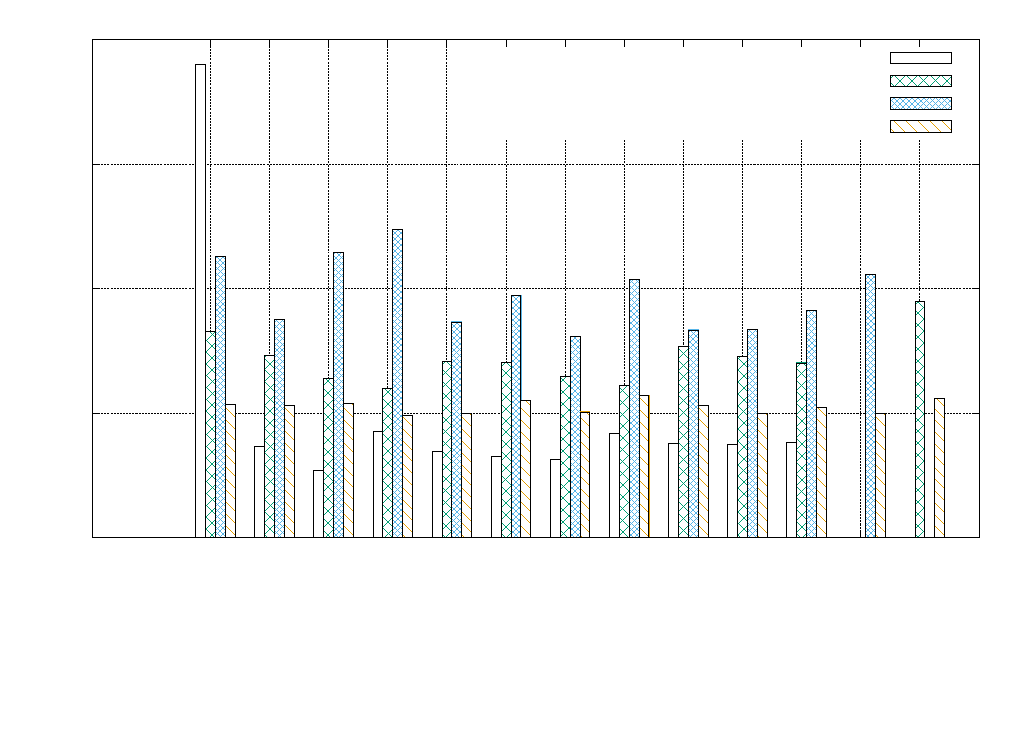
\includegraphics{./Results/Feature_Permutation/statereg_ratio.eps}}%
    \gplfronttext
  \end{picture}%
\endgroup

	\label{fig:State Register Ratio ($SRR_n$) Per Feature}
}
\end{frame}

\begin{frame}{Feature Occurrence --- Method 2}
\begin{itemize}
	\item Removing features using Table \ref{tab: conditions for filtering}
	\item Count total number of times feature appear across all implementation per file
	\item Average Count and Normalize
\end{itemize}
\begin{table}[ht]
	\centering
   \begin{tabular}{|c|c|}
   	\hline
       $A_{original}<A_{permuted}$ & Feature Hindrance\\
       \hline
       $A_{original}=A_{permuted}$ & Feature Hindrance\\
       \hline
       $A_{original}>A_{permuted}$, \; with a difference of $> 1\%$  & Feature Important\\
       \hline
  \end{tabular}
  \caption{Conditions for filtering}
  \label{tab: conditions for filtering}
\end{table}
\end{frame}

\begin{frame}{Feature Permutation Method 2 \\Model Feature Occurrence}
\centering
\resizebox{!}{0.7\paperheight}{
	% GNUPLOT: LaTeX picture with Postscript
\begingroup
  \makeatletter
  \providecommand\color[2][]{%
    \GenericError{(gnuplot) \space\space\space\@spaces}{%
      Package color not loaded in conjunction with
      terminal option `colourtext'%
    }{See the gnuplot documentation for explanation.%
    }{Either use 'blacktext' in gnuplot or load the package
      color.sty in LaTeX.}%
    \renewcommand\color[2][]{}%
  }%
  \providecommand\includegraphics[2][]{%
    \GenericError{(gnuplot) \space\space\space\@spaces}{%
      Package graphicx or graphics not loaded%
    }{See the gnuplot documentation for explanation.%
    }{The gnuplot epslatex terminal needs graphicx.sty or graphics.sty.}%
    \renewcommand\includegraphics[2][]{}%
  }%
  \providecommand\rotatebox[2]{#2}%
  \@ifundefined{ifGPcolor}{%
    \newif\ifGPcolor
    \GPcolortrue
  }{}%
  \@ifundefined{ifGPblacktext}{%
    \newif\ifGPblacktext
    \GPblacktexttrue
  }{}%
  % define a \g@addto@macro without @ in the name:
  \let\gplgaddtomacro\g@addto@macro
  % define empty templates for all commands taking text:
  \gdef\gplbacktext{}%
  \gdef\gplfronttext{}%
  \makeatother
  \ifGPblacktext
    % no textcolor at all
    \def\colorrgb#1{}%
    \def\colorgray#1{}%
  \else
    % gray or color?
    \ifGPcolor
      \def\colorrgb#1{\color[rgb]{#1}}%
      \def\colorgray#1{\color[gray]{#1}}%
      \expandafter\def\csname LTw\endcsname{\color{white}}%
      \expandafter\def\csname LTb\endcsname{\color{black}}%
      \expandafter\def\csname LTa\endcsname{\color{black}}%
      \expandafter\def\csname LT0\endcsname{\color[rgb]{1,0,0}}%
      \expandafter\def\csname LT1\endcsname{\color[rgb]{0,1,0}}%
      \expandafter\def\csname LT2\endcsname{\color[rgb]{0,0,1}}%
      \expandafter\def\csname LT3\endcsname{\color[rgb]{1,0,1}}%
      \expandafter\def\csname LT4\endcsname{\color[rgb]{0,1,1}}%
      \expandafter\def\csname LT5\endcsname{\color[rgb]{1,1,0}}%
      \expandafter\def\csname LT6\endcsname{\color[rgb]{0,0,0}}%
      \expandafter\def\csname LT7\endcsname{\color[rgb]{1,0.3,0}}%
      \expandafter\def\csname LT8\endcsname{\color[rgb]{0.5,0.5,0.5}}%
    \else
      % gray
      \def\colorrgb#1{\color{black}}%
      \def\colorgray#1{\color[gray]{#1}}%
      \expandafter\def\csname LTw\endcsname{\color{white}}%
      \expandafter\def\csname LTb\endcsname{\color{black}}%
      \expandafter\def\csname LTa\endcsname{\color{black}}%
      \expandafter\def\csname LT0\endcsname{\color{black}}%
      \expandafter\def\csname LT1\endcsname{\color{black}}%
      \expandafter\def\csname LT2\endcsname{\color{black}}%
      \expandafter\def\csname LT3\endcsname{\color{black}}%
      \expandafter\def\csname LT4\endcsname{\color{black}}%
      \expandafter\def\csname LT5\endcsname{\color{black}}%
      \expandafter\def\csname LT6\endcsname{\color{black}}%
      \expandafter\def\csname LT7\endcsname{\color{black}}%
      \expandafter\def\csname LT8\endcsname{\color{black}}%
    \fi
  \fi
    \setlength{\unitlength}{0.0500bp}%
    \ifx\gptboxheight\undefined%
      \newlength{\gptboxheight}%
      \newlength{\gptboxwidth}%
      \newsavebox{\gptboxtext}%
    \fi%
    \setlength{\fboxrule}{0.5pt}%
    \setlength{\fboxsep}{1pt}%
\begin{picture}(9636.00,6802.00)%
    \gplgaddtomacro\gplbacktext{%
      \csname LTb\endcsname%%
      \put(594,1803){\makebox(0,0)[r]{\strut{}$0.2$}}%
      \csname LTb\endcsname%%
      \put(594,2759){\makebox(0,0)[r]{\strut{}$0.4$}}%
      \csname LTb\endcsname%%
      \put(594,3714){\makebox(0,0)[r]{\strut{}$0.6$}}%
      \csname LTb\endcsname%%
      \put(594,4670){\makebox(0,0)[r]{\strut{}$0.8$}}%
      \csname LTb\endcsname%%
      \put(594,5625){\makebox(0,0)[r]{\strut{}$1$}}%
      \csname LTb\endcsname%%
      \put(594,6581){\makebox(0,0)[r]{\strut{}$1.2$}}%
      \csname LTb\endcsname%%
      \put(1861,1671){\rotatebox{30}{\makebox(0,0)[r]{\strut{}average neighbour degree}}}%
      \csname LTb\endcsname%%
      \put(2429,1671){\rotatebox{30}{\makebox(0,0)[r]{\strut{}betweenness centrality}}}%
      \csname LTb\endcsname%%
      \put(2996,1671){\rotatebox{30}{\makebox(0,0)[r]{\strut{}closeness centrality}}}%
      \csname LTb\endcsname%%
      \put(3564,1671){\rotatebox{30}{\makebox(0,0)[r]{\strut{}clustering}}}%
      \csname LTb\endcsname%%
      \put(4131,1671){\rotatebox{30}{\makebox(0,0)[r]{\strut{}degree}}}%
      \csname LTb\endcsname%%
      \put(4699,1671){\rotatebox{30}{\makebox(0,0)[r]{\strut{}degree centrality}}}%
      \csname LTb\endcsname%%
      \put(5266,1671){\rotatebox{30}{\makebox(0,0)[r]{\strut{}has feedback path}}}%
      \csname LTb\endcsname%%
      \put(5834,1671){\rotatebox{30}{\makebox(0,0)[r]{\strut{}katz}}}%
      \csname LTb\endcsname%%
      \put(6401,1671){\rotatebox{30}{\makebox(0,0)[r]{\strut{}load centrality}}}%
      \csname LTb\endcsname%%
      \put(6969,1671){\rotatebox{30}{\makebox(0,0)[r]{\strut{}outdegree}}}%
      \csname LTb\endcsname%%
      \put(7536,1671){\rotatebox{30}{\makebox(0,0)[r]{\strut{}pagerank}}}%
      \csname LTb\endcsname%%
      \put(8104,1671){\rotatebox{30}{\makebox(0,0)[r]{\strut{}euclidean}}}%
      \csname LTb\endcsname%%
      \put(8671,1671){\rotatebox{30}{\makebox(0,0)[r]{\strut{}fastRELIC}}}%
    }%
    \gplgaddtomacro\gplfronttext{%
      \csname LTb\endcsname%%
      \put(8252,6408){\makebox(0,0)[r]{\strut{}Original}}%
      \csname LTb\endcsname%%
      \put(8252,6188){\makebox(0,0)[r]{\strut{}With fastRELIC}}%
      \csname LTb\endcsname%%
      \put(8252,5968){\makebox(0,0)[r]{\strut{}With Euclidean}}%
      \csname LTb\endcsname%%
      \put(8252,5748){\makebox(0,0)[r]{\strut{}With Euclidean and fastRELIC}}%
    }%
    \gplbacktext
    \put(0,0){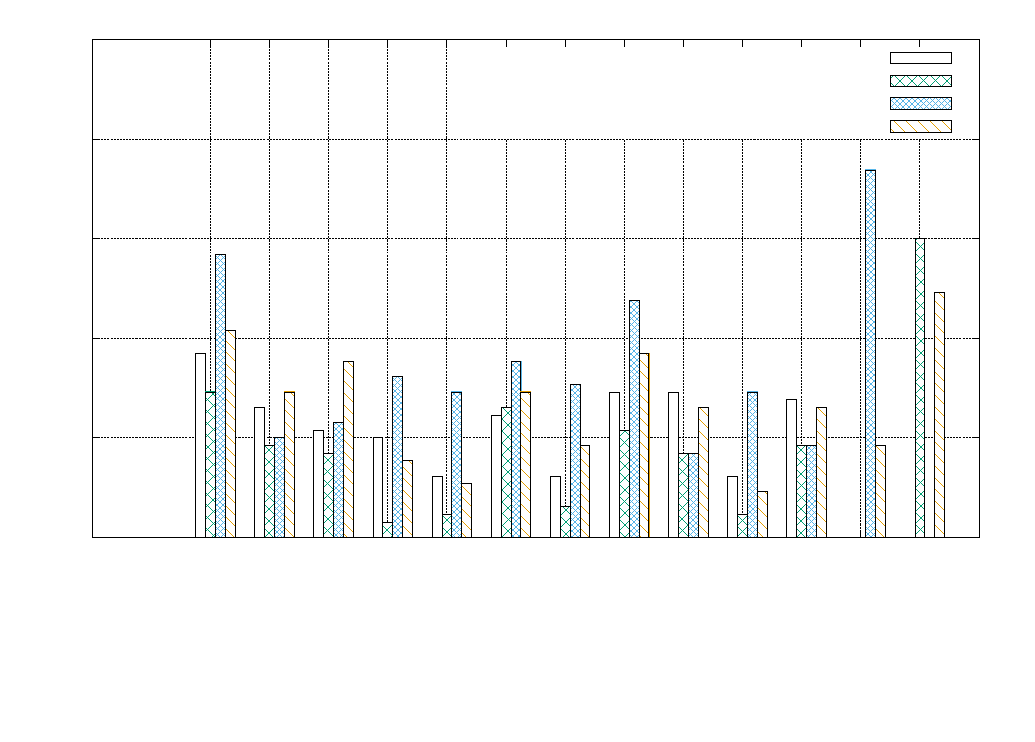
\includegraphics{FeaturePermutation_count}}%
    \gplfronttext
  \end{picture}%
\endgroup

	\label{fig:Feature Occurrence Percentage: FP Model}
}
\end{frame}

\begin{frame}{Feature Permutation Method 2 \\State Register Feature Occurrence}
\centering
\resizebox{!}{0.7\paperheight}{
% GNUPLOT: LaTeX picture with Postscript
\begingroup
  \makeatletter
  \providecommand\color[2][]{%
    \GenericError{(gnuplot) \space\space\space\@spaces}{%
      Package color not loaded in conjunction with
      terminal option `colourtext'%
    }{See the gnuplot documentation for explanation.%
    }{Either use 'blacktext' in gnuplot or load the package
      color.sty in LaTeX.}%
    \renewcommand\color[2][]{}%
  }%
  \providecommand\includegraphics[2][]{%
    \GenericError{(gnuplot) \space\space\space\@spaces}{%
      Package graphicx or graphics not loaded%
    }{See the gnuplot documentation for explanation.%
    }{The gnuplot epslatex terminal needs graphicx.sty or graphics.sty.}%
    \renewcommand\includegraphics[2][]{}%
  }%
  \providecommand\rotatebox[2]{#2}%
  \@ifundefined{ifGPcolor}{%
    \newif\ifGPcolor
    \GPcolortrue
  }{}%
  \@ifundefined{ifGPblacktext}{%
    \newif\ifGPblacktext
    \GPblacktexttrue
  }{}%
  % define a \g@addto@macro without @ in the name:
  \let\gplgaddtomacro\g@addto@macro
  % define empty templates for all commands taking text:
  \gdef\gplbacktext{}%
  \gdef\gplfronttext{}%
  \makeatother
  \ifGPblacktext
    % no textcolor at all
    \def\colorrgb#1{}%
    \def\colorgray#1{}%
  \else
    % gray or color?
    \ifGPcolor
      \def\colorrgb#1{\color[rgb]{#1}}%
      \def\colorgray#1{\color[gray]{#1}}%
      \expandafter\def\csname LTw\endcsname{\color{white}}%
      \expandafter\def\csname LTb\endcsname{\color{black}}%
      \expandafter\def\csname LTa\endcsname{\color{black}}%
      \expandafter\def\csname LT0\endcsname{\color[rgb]{1,0,0}}%
      \expandafter\def\csname LT1\endcsname{\color[rgb]{0,1,0}}%
      \expandafter\def\csname LT2\endcsname{\color[rgb]{0,0,1}}%
      \expandafter\def\csname LT3\endcsname{\color[rgb]{1,0,1}}%
      \expandafter\def\csname LT4\endcsname{\color[rgb]{0,1,1}}%
      \expandafter\def\csname LT5\endcsname{\color[rgb]{1,1,0}}%
      \expandafter\def\csname LT6\endcsname{\color[rgb]{0,0,0}}%
      \expandafter\def\csname LT7\endcsname{\color[rgb]{1,0.3,0}}%
      \expandafter\def\csname LT8\endcsname{\color[rgb]{0.5,0.5,0.5}}%
    \else
      % gray
      \def\colorrgb#1{\color{black}}%
      \def\colorgray#1{\color[gray]{#1}}%
      \expandafter\def\csname LTw\endcsname{\color{white}}%
      \expandafter\def\csname LTb\endcsname{\color{black}}%
      \expandafter\def\csname LTa\endcsname{\color{black}}%
      \expandafter\def\csname LT0\endcsname{\color{black}}%
      \expandafter\def\csname LT1\endcsname{\color{black}}%
      \expandafter\def\csname LT2\endcsname{\color{black}}%
      \expandafter\def\csname LT3\endcsname{\color{black}}%
      \expandafter\def\csname LT4\endcsname{\color{black}}%
      \expandafter\def\csname LT5\endcsname{\color{black}}%
      \expandafter\def\csname LT6\endcsname{\color{black}}%
      \expandafter\def\csname LT7\endcsname{\color{black}}%
      \expandafter\def\csname LT8\endcsname{\color{black}}%
    \fi
  \fi
    \setlength{\unitlength}{0.0500bp}%
    \ifx\gptboxheight\undefined%
      \newlength{\gptboxheight}%
      \newlength{\gptboxwidth}%
      \newsavebox{\gptboxtext}%
    \fi%
    \setlength{\fboxrule}{0.5pt}%
    \setlength{\fboxsep}{1pt}%
\begin{picture}(9636.00,6802.00)%
    \gplgaddtomacro\gplbacktext{%
      \csname LTb\endcsname%%
      \put(594,1803){\makebox(0,0)[r]{\strut{}$0$}}%
      \csname LTb\endcsname%%
      \put(594,2759){\makebox(0,0)[r]{\strut{}$0.2$}}%
      \csname LTb\endcsname%%
      \put(594,3714){\makebox(0,0)[r]{\strut{}$0.4$}}%
      \csname LTb\endcsname%%
      \put(594,4670){\makebox(0,0)[r]{\strut{}$0.6$}}%
      \csname LTb\endcsname%%
      \put(594,5625){\makebox(0,0)[r]{\strut{}$0.8$}}%
      \csname LTb\endcsname%%
      \put(594,6581){\makebox(0,0)[r]{\strut{}$1$}}%
      \csname LTb\endcsname%%
      \put(1861,1671){\rotatebox{30}{\makebox(0,0)[r]{\strut{}average neighbour degree}}}%
      \csname LTb\endcsname%%
      \put(2429,1671){\rotatebox{30}{\makebox(0,0)[r]{\strut{}betweenness centrality}}}%
      \csname LTb\endcsname%%
      \put(2996,1671){\rotatebox{30}{\makebox(0,0)[r]{\strut{}closeness centrality}}}%
      \csname LTb\endcsname%%
      \put(3564,1671){\rotatebox{30}{\makebox(0,0)[r]{\strut{}clustering}}}%
      \csname LTb\endcsname%%
      \put(4131,1671){\rotatebox{30}{\makebox(0,0)[r]{\strut{}degree}}}%
      \csname LTb\endcsname%%
      \put(4699,1671){\rotatebox{30}{\makebox(0,0)[r]{\strut{}degree centrality}}}%
      \csname LTb\endcsname%%
      \put(5266,1671){\rotatebox{30}{\makebox(0,0)[r]{\strut{}has feedback path}}}%
      \csname LTb\endcsname%%
      \put(5834,1671){\rotatebox{30}{\makebox(0,0)[r]{\strut{}katz}}}%
      \csname LTb\endcsname%%
      \put(6401,1671){\rotatebox{30}{\makebox(0,0)[r]{\strut{}load centrality}}}%
      \csname LTb\endcsname%%
      \put(6969,1671){\rotatebox{30}{\makebox(0,0)[r]{\strut{}outdegree}}}%
      \csname LTb\endcsname%%
      \put(7536,1671){\rotatebox{30}{\makebox(0,0)[r]{\strut{}pagerank}}}%
      \csname LTb\endcsname%%
      \put(8104,1671){\rotatebox{30}{\makebox(0,0)[r]{\strut{}euclidean}}}%
      \csname LTb\endcsname%%
      \put(8671,1671){\rotatebox{30}{\makebox(0,0)[r]{\strut{}fastRELIC}}}%
    }%
    \gplgaddtomacro\gplfronttext{%
      \csname LTb\endcsname%%
      \put(8252,6408){\makebox(0,0)[r]{\strut{}Original}}%
      \csname LTb\endcsname%%
      \put(8252,6188){\makebox(0,0)[r]{\strut{}With fastRELIC}}%
      \csname LTb\endcsname%%
      \put(8252,5968){\makebox(0,0)[r]{\strut{}With Euclidean}}%
      \csname LTb\endcsname%%
      \put(8252,5748){\makebox(0,0)[r]{\strut{}With Euclidean and fastRELIC}}%
    }%
    \gplbacktext
    \put(0,0){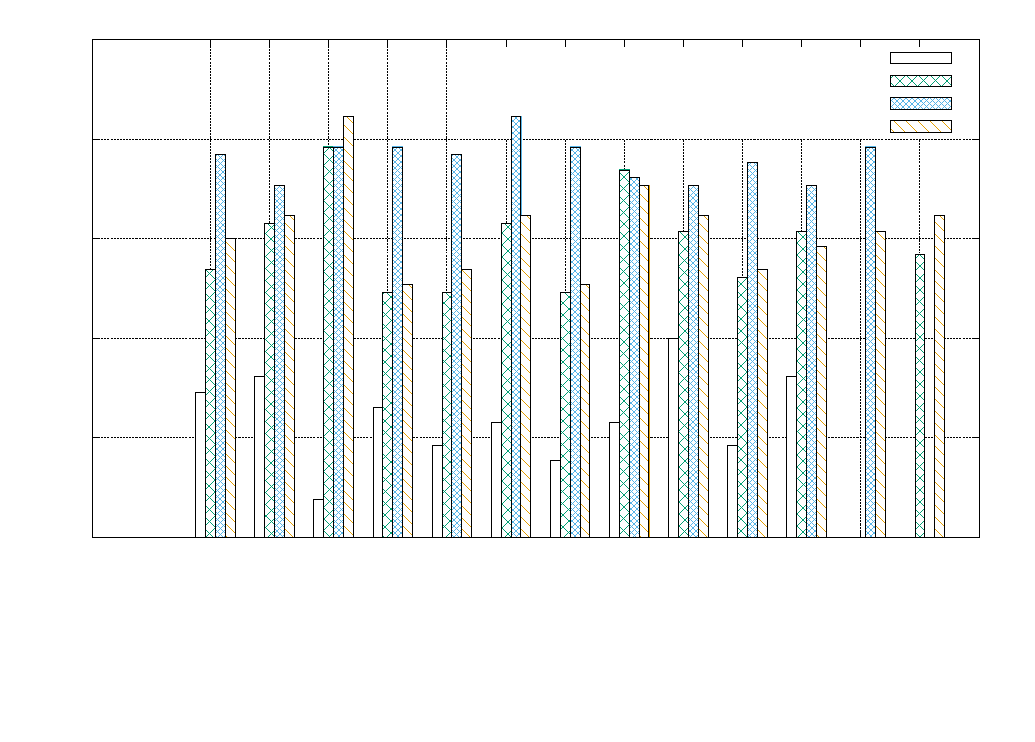
\includegraphics{myFiles/myLatex/Feature_Permutation/statereg_counter.eps}}%
    \gplfronttext
  \end{picture}%
\endgroup

\label{fig:Feature Occurrence Percentage: FP State Register}
}
\end{frame}

\begin{frame}{Sequential Feature Selection}
\begin{itemize}
	\item Rotation of 13 files, 12 for training, 1 for testing
	\item Run 5 times per file per implementation
	\item Count occurence per feature across all files
	\item Count total number of times feature appear across all implementation per file
	\item Average Count and Normalize
	\item Discard Feature Occuring $<50\%$
\end{itemize}
\end{frame}

\begin{frame}{Sequential Feature Selection}
\centering
\resizebox{!}{0.7\paperheight}{
	% GNUPLOT: LaTeX picture with Postscript
\begingroup
  \makeatletter
  \providecommand\color[2][]{%
    \GenericError{(gnuplot) \space\space\space\@spaces}{%
      Package color not loaded in conjunction with
      terminal option `colourtext'%
    }{See the gnuplot documentation for explanation.%
    }{Either use 'blacktext' in gnuplot or load the package
      color.sty in LaTeX.}%
    \renewcommand\color[2][]{}%
  }%
  \providecommand\includegraphics[2][]{%
    \GenericError{(gnuplot) \space\space\space\@spaces}{%
      Package graphicx or graphics not loaded%
    }{See the gnuplot documentation for explanation.%
    }{The gnuplot epslatex terminal needs graphicx.sty or graphics.sty.}%
    \renewcommand\includegraphics[2][]{}%
  }%
  \providecommand\rotatebox[2]{#2}%
  \@ifundefined{ifGPcolor}{%
    \newif\ifGPcolor
    \GPcolortrue
  }{}%
  \@ifundefined{ifGPblacktext}{%
    \newif\ifGPblacktext
    \GPblacktexttrue
  }{}%
  % define a \g@addto@macro without @ in the name:
  \let\gplgaddtomacro\g@addto@macro
  % define empty templates for all commands taking text:
  \gdef\gplbacktext{}%
  \gdef\gplfronttext{}%
  \makeatother
  \ifGPblacktext
    % no textcolor at all
    \def\colorrgb#1{}%
    \def\colorgray#1{}%
  \else
    % gray or color?
    \ifGPcolor
      \def\colorrgb#1{\color[rgb]{#1}}%
      \def\colorgray#1{\color[gray]{#1}}%
      \expandafter\def\csname LTw\endcsname{\color{white}}%
      \expandafter\def\csname LTb\endcsname{\color{black}}%
      \expandafter\def\csname LTa\endcsname{\color{black}}%
      \expandafter\def\csname LT0\endcsname{\color[rgb]{1,0,0}}%
      \expandafter\def\csname LT1\endcsname{\color[rgb]{0,1,0}}%
      \expandafter\def\csname LT2\endcsname{\color[rgb]{0,0,1}}%
      \expandafter\def\csname LT3\endcsname{\color[rgb]{1,0,1}}%
      \expandafter\def\csname LT4\endcsname{\color[rgb]{0,1,1}}%
      \expandafter\def\csname LT5\endcsname{\color[rgb]{1,1,0}}%
      \expandafter\def\csname LT6\endcsname{\color[rgb]{0,0,0}}%
      \expandafter\def\csname LT7\endcsname{\color[rgb]{1,0.3,0}}%
      \expandafter\def\csname LT8\endcsname{\color[rgb]{0.5,0.5,0.5}}%
    \else
      % gray
      \def\colorrgb#1{\color{black}}%
      \def\colorgray#1{\color[gray]{#1}}%
      \expandafter\def\csname LTw\endcsname{\color{white}}%
      \expandafter\def\csname LTb\endcsname{\color{black}}%
      \expandafter\def\csname LTa\endcsname{\color{black}}%
      \expandafter\def\csname LT0\endcsname{\color{black}}%
      \expandafter\def\csname LT1\endcsname{\color{black}}%
      \expandafter\def\csname LT2\endcsname{\color{black}}%
      \expandafter\def\csname LT3\endcsname{\color{black}}%
      \expandafter\def\csname LT4\endcsname{\color{black}}%
      \expandafter\def\csname LT5\endcsname{\color{black}}%
      \expandafter\def\csname LT6\endcsname{\color{black}}%
      \expandafter\def\csname LT7\endcsname{\color{black}}%
      \expandafter\def\csname LT8\endcsname{\color{black}}%
    \fi
  \fi
    \setlength{\unitlength}{0.0500bp}%
    \ifx\gptboxheight\undefined%
      \newlength{\gptboxheight}%
      \newlength{\gptboxwidth}%
      \newsavebox{\gptboxtext}%
    \fi%
    \setlength{\fboxrule}{0.5pt}%
    \setlength{\fboxsep}{1pt}%
\begin{picture}(9636.00,6802.00)%
    \gplgaddtomacro\gplbacktext{%
      \csname LTb\endcsname%%
      \put(594,1803){\makebox(0,0)[r]{\strut{}$0.2$}}%
      \csname LTb\endcsname%%
      \put(594,2759){\makebox(0,0)[r]{\strut{}$0.4$}}%
      \csname LTb\endcsname%%
      \put(594,3714){\makebox(0,0)[r]{\strut{}$0.6$}}%
      \csname LTb\endcsname%%
      \put(594,4670){\makebox(0,0)[r]{\strut{}$0.8$}}%
      \csname LTb\endcsname%%
      \put(594,5625){\makebox(0,0)[r]{\strut{}$1$}}%
      \csname LTb\endcsname%%
      \put(594,6581){\makebox(0,0)[r]{\strut{}$1.2$}}%
      \csname LTb\endcsname%%
      \put(1861,1671){\rotatebox{30}{\makebox(0,0)[r]{\strut{}average neighbour degree}}}%
      \csname LTb\endcsname%%
      \put(2429,1671){\rotatebox{30}{\makebox(0,0)[r]{\strut{}betweenness centrality}}}%
      \csname LTb\endcsname%%
      \put(2996,1671){\rotatebox{30}{\makebox(0,0)[r]{\strut{}closeness centrality}}}%
      \csname LTb\endcsname%%
      \put(3564,1671){\rotatebox{30}{\makebox(0,0)[r]{\strut{}clustering}}}%
      \csname LTb\endcsname%%
      \put(4131,1671){\rotatebox{30}{\makebox(0,0)[r]{\strut{}degree}}}%
      \csname LTb\endcsname%%
      \put(4699,1671){\rotatebox{30}{\makebox(0,0)[r]{\strut{}degree centrality}}}%
      \csname LTb\endcsname%%
      \put(5266,1671){\rotatebox{30}{\makebox(0,0)[r]{\strut{}has feedback path}}}%
      \csname LTb\endcsname%%
      \put(5834,1671){\rotatebox{30}{\makebox(0,0)[r]{\strut{}katz}}}%
      \csname LTb\endcsname%%
      \put(6401,1671){\rotatebox{30}{\makebox(0,0)[r]{\strut{}load centrality}}}%
      \csname LTb\endcsname%%
      \put(6969,1671){\rotatebox{30}{\makebox(0,0)[r]{\strut{}outdegree}}}%
      \csname LTb\endcsname%%
      \put(7536,1671){\rotatebox{30}{\makebox(0,0)[r]{\strut{}pagerank}}}%
      \csname LTb\endcsname%%
      \put(8104,1671){\rotatebox{30}{\makebox(0,0)[r]{\strut{}euclidean}}}%
      \csname LTb\endcsname%%
      \put(8671,1671){\rotatebox{30}{\makebox(0,0)[r]{\strut{}fastRELIC}}}%
    }%
    \gplgaddtomacro\gplfronttext{%
      \csname LTb\endcsname%%
      \put(8252,6408){\makebox(0,0)[r]{\strut{}Original}}%
      \csname LTb\endcsname%%
      \put(8252,6188){\makebox(0,0)[r]{\strut{}With fastRELIC}}%
      \csname LTb\endcsname%%
      \put(8252,5968){\makebox(0,0)[r]{\strut{}With Euclidean}}%
      \csname LTb\endcsname%%
      \put(8252,5748){\makebox(0,0)[r]{\strut{}With Euclidean and fastRELIC}}%
    }%
    \gplbacktext
    \put(0,0){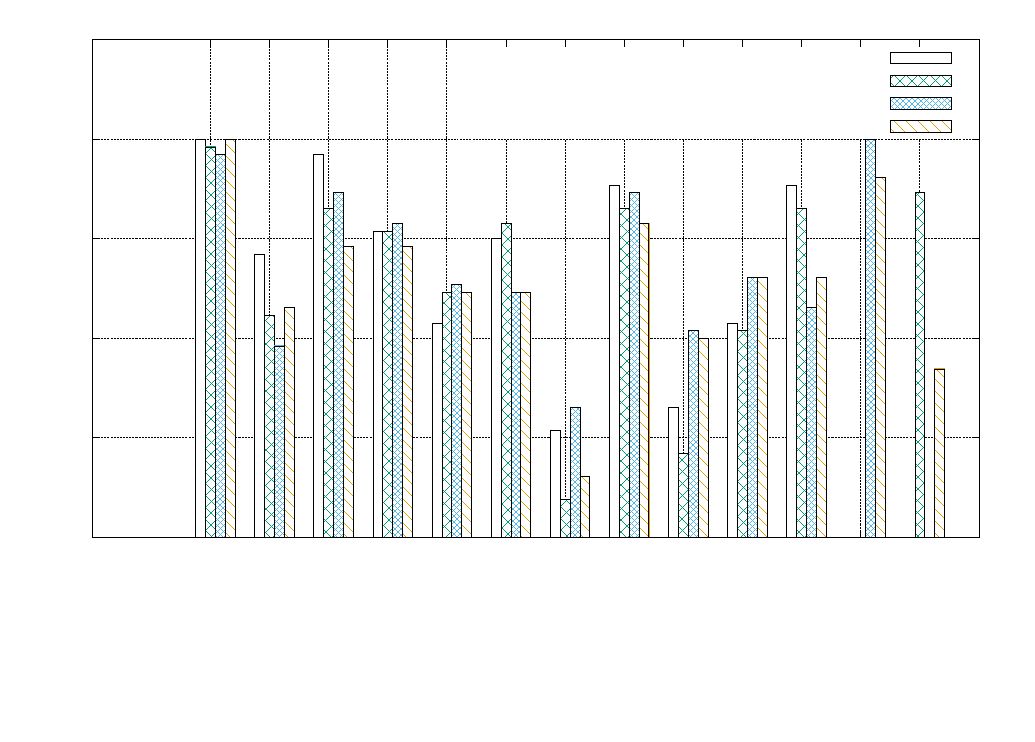
\includegraphics{SFS}}%
    \gplfronttext
  \end{picture}%
\endgroup

	\label{fig:Feature Occurrence Percentage: SFS}
}
\end{frame}

\begin{frame}{Conclusion for feature selection}
Important Features
	\begin{itemize}
		\item Average Neighbour Degree
		\item Katz
	\end{itemize}
Redundant Features
\begin{itemize}
	\item Has Feedback Path
	\item Load Centrality
\end{itemize}
\end{frame}


\begin{frame}{Results after Removing Features}
\centering
\begin{table}
	\begin{tabular}{|c|c|c|}
		\hline
		Implementation & Mean Model Acc & Mean State Register Acc\\
		\hline
	  	\hline
		Original & 0.75 & 0.59\\
		\hline
		With fastRELIC & 0.86 & 0.77\\
		\hline
		With Euclidean & 0.83 & 0.70\\
		\hline
		With Euclidean and fastRELIC & 0.87 & 0.77\\
  		\hline
	\end{tabular}
	\caption{Model Accuracy}
	\label{tab:Accuracy after feature selection}
\end{table}
\end{frame}

\begin{frame}[c]{ }
\begin{center}
	\Huge Optimizing
\end{center}
\end{frame}

\begin{frame}{Optimized Model Accuracy}
\centering
\begin{table}
	\begin{tabular}{|c|c|}
		\hline
		Mean Model Acc & Mean State Register Acc\\
		\hline
	  	\hline
		0.65 & 0.91\\
  		\hline
	\end{tabular}
	\caption{Optimized Model Accuracy}
	\label{tab:Optimized Model Accuracy}
\end{table}
\begin{itemize}
	\item Low Model Accuracy --- High False Positive
	\item Model is Underfitted --- Epoch might be too low
\end{itemize}
\end{frame}

\begin{frame}{Further tuning the Optimized Model}
\begin{itemize}
	\item Increasing the Epochs from 10 to 22
\end{itemize}
\centering
\begin{table}
	\begin{tabular}{|c|c|}
		\hline
		Mean Model Acc & Mean State Register Acc\\
		\hline
	  	\hline
		0.75 & 0.91\\
  		\hline
	\end{tabular}
	\caption{Modified Optimized Model Accuracy}
	\label{tab:Modified Optimized Model Accuracy}
\end{table}
\end{frame}

\section{Future Work}
\begin{frame}{Future Work}
	\begin{itemize}
		\item Using a larger data set
		\item Studying feature Correlation
		\item Using other feature selection method, eg. exhaustive feature selection
		\item Removing dependency on registers per file
		\item Experimenting with other Neural Network Architecture and hyperparameters
	\end{itemize}
\end{frame}

\begin{frame}[c]{ }
	\begin{center}
		\Huge Thank You
	\end{center}
\end{frame}


\begin{frame}{Register shape}
\begin{figure}
	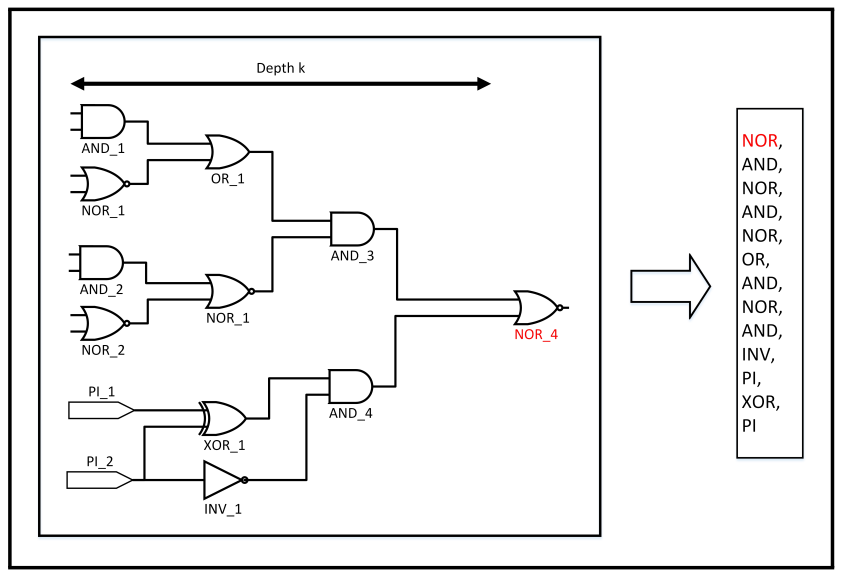
\includegraphics[scale=0.3]{./Results/vector/register_shape.png}
\end{figure}
\end{frame}


\end{document}




